\documentclass[a0paper,portrait,fontscale=0.40]{baposter}



\usepackage[export]{adjustbox} % Nice alternative to minipage.
\usepackage{afterpage} % To give the title page its own geometry.
\usepackage{amsmath} % Nice maths symbols.
\usepackage{amssymb} % Nice variable symbols.
\usepackage{array} % Allow for custom column widths in tables.
\usepackage{ltablex} % For long tables spanning multiple pages. % Must be before ARYDSHLN package!
\keepXColumns % Keeps the X column
\usepackage{colortbl} % Gives table colours. % Must be before ARYDSHLN package!
\usepackage{arydshln} % Dashed lines using \hdashline \cdashline
\usepackage{bbm} % Gives Blackboard fonts.
\usepackage{blindtext} % Gives dummy text / maths.
\usepackage{bm} % Bold math symbols.
\usepackage{calc} % Calculates widths of words. 
\usepackage{chngcntr} % Changing counters, e.g. with footnotes.
\usepackage[final]{draftwatermark} % Gives a draft overlay. Use options [nostamp] or [final].
\usepackage{emptypage} % Empty pages have no headers and footers.
\usepackage[shortlabels]{enumitem} % Nice listing options in itemize and enumerate.
\usepackage{esdiff} % Gives nice differential operators.
\usepackage{esvect} % Gives nice vector arrows.
%\usepackage{fancyhdr} % Nice headers.
\usepackage{float} % Nice figure placement.
\usepackage[T1]{fontenc} % Nice range of text characters and accents.
\usepackage[bottom]{footmisc} % Nice footnote formatting.
\usepackage{graphicx} % Include figures.
%\usepackage[notquote]{hanging} % For indenting later lines in a paragraph. USE the 'noquote' option else the `'` is overwritten, and breaks in maths mode!
\usepackage{ifoddpage} % Checks for odd or even page.
%\usepackage{imakeidx} % Makes the index.
\usepackage{indentfirst} % Indents the first paragraph.
\usepackage{letltxmacro} % For defining a nice SQRT symbol.
\usepackage{lipsum} % Useful for adding jargon.
%\usepackage{listings} % The listings package for code.
\usepackage{lmodern} % Load a font with all the characters
\usepackage{marginnote} % For nice margin notes.
\usepackage{mathtools} % Gives the colon equals symbol.
\usepackage[framed,numbered,autolinebreaks,useliterate]{mcode} % Inports Listings package ideal for MATLAB.
\usepackage[framemethod=tikz]{mdframed} % Gives nices boxed and sidesrules.
\usepackage{multirow} % Nice table cells spanning many rows.
\usepackage{multicol} % If I want to use multiple columns.
\usepackage[numbers, sort&compress]{natbib} % Nice references.
\usepackage{nicefrac} % Gives nice fractions for superscripts.
%\usepackage{nomencl} % Gives a symbol nomenclature. 
\usepackage[super]{nth} % Gives nice ordinal superscripts, eg 1st, 2nd, etc.
%\usepackage{parskip} % Gives nicer indenting.
\usepackage{physics} % Nice partial derivatives and BRAKET notation.
\usepackage{ragged2e} % For nice allignment.
%\usepackage[norefs]{refcheck} % Can show any unused references.
\usepackage{romannum} % Nice typing for roman numerals.
\usepackage{setspace} % Ideal for increasing line spacing. E.g.  \doublespacing
\usepackage{siunitx} % Nice formating of units.
\usepackage{sidenotes} % Nice margin figures and margin tables. 
\usepackage{subcaption} % Side by side figures.
\usepackage[textsize=tiny]{todonotes} % A nice TODO list. [disable] to supress.
\usepackage{tikz} % Nice diagrams.
%\usepackage[nottoc]{tocbibind} % Gives nices Table of Contents
%\usepackage[table]{xcolor} % This is useful for making greyed table cells, nice for headers. Known preamble placement issues.
\usepackage{wasysym} % Gives some nice misc symbols, such as markers.
\usepackage{wrapfig} % Allows wrapping text around figures. 
\usepackage{xifthen}% Provides \isempty test.
\usepackage{xparse} % Gives \NewDocumentEnvironment which has nice optional argument handling.
\usepackage{xspace} % Gives nice spacing for commands.
%%%% Generally HYPERREF should be imported last. %%%%
\usepackage[colorlinks=true,linkcolor=black,urlcolor=black,citecolor=black,anchorcolor=black]{hyperref} % Colour links.
%%%% Should be loaded after hyperref. %%%%
\usepackage{cleveref} % Gives smart referencing. %% After Hyperref
\usepackage[margin=10pt,font=small,labelfont=bf,labelsep=endash,figurewithin=section,tablewithin=section]{caption} % Caption figures and tables nicely. %% After cleveref.
%\usepackage{geometry} % Use nice margins. Does give a small change in the default page margins. 

% Enable dummy maths
\blindmathtrue


%\hbadness=10000 % Supresses bad box warnings

% Where to search for figures. 
\graphicspath{{../../figures/}{../../figures/hardware/}{../../figures/inverse_cdf/}{../../figures/logos/}{../../papers/}{../../figures_remote/}}

% Present the references in the order they are used.
\bibliographystyle{unsrtnattruncated}
% Reduce spacing between references. 
\setlength{\bibsep}{0pt plus 0.3ex}


% Listing -> Code in environment labels.
\renewcommand{\lstlistingname}{Code}

% Nice paragraph indents.
%\setlength{\parindent}{15mm}

% Giving the references the right title.
\renewcommand{\bibname}{References}

% Removes hyphenation
\tolerance=1
\emergencystretch=\maxdimen
\hyphenpenalty=10000
\hbadness=10000

% To change the spacing in lists
\setlist{noitemsep} % or \setlist{noitemsep} to leave space around whole list
%\setenumerate{itemsep=-0.4em,topsep=0.5em} % Seems to look nice.

% Custom column widths using C{2cm}, L, R, etc.
\newcolumntype{L}[1]{>{\raggedright\let\newline\\\arraybackslash\hspace{0pt}}m{#1}}
\newcolumntype{C}[1]{>{\centering\let\newline\\\arraybackslash\hspace{0pt}}m{#1}}
\newcolumntype{R}[1]{>{\raggedleft\let\newline\\\arraybackslash\hspace{0pt}}m{#1}}

% Gives a nice column separation in multicolumn mode.
\setlength{\columnsep}{5mm}

% Figure environment for use in multicolumn. To put in captions use \captionof{figure}{content of caption}.
\newenvironment{Figure}
{\par\medskip\noindent\minipage{\linewidth}}
{\endminipage\par\medskip}

% Gives the nice SQRT symbol.
\makeatletter
\let\oldr@@t\r@@t
\def\r@@t#1#2{%
	\setbox0=\hbox{$\oldr@@t#1{#2\,}$}\dimen0=\ht0
	\advance\dimen0-0.2\ht0
	\setbox2=\hbox{\vrule height\ht0 depth -\dimen0}%
	{\box0\lower0.4pt\box2}}
\LetLtxMacro{\oldsqrt}{\sqrt}
\renewcommand*{\sqrt}[2][\ ]{\oldsqrt[#1]{#2}}
\makeatother

\DeclareMathOperator{\sign}{sign}
%\DeclareMathOperator{\erf}{erf}
\DeclareMathOperator*{\argmin}{argmin}
\DeclareMathOperator*{\argmax}{argmax}
% Number equations down to the subection level, e.g. 1.2.3 is the third equation in
% subsection 2 of section 1.
%\numberwithin{equation}{section}
\newcommand*\tageq{\refstepcounter{equation}\tag{\theequation}}

% Nice spacing in the first row of a table
\newcommand{\firstrowspacing}{\rule{0pt}{2.6ex}}
% For a more open look in tables.
\setlength\extrarowheight{3pt} 

% Some corporate names we may need to append a \textsuperscript{\textregistered} into. 
\newcommand{\nag}{NAG\xspace}
\newcommand{\arm}{Arm\xspace}
\newcommand{\intel}{Intel\xspace}
\newcommand{\amd}{AMD\xspace}
\newcommand{\ibm}{IBM\xspace}
\newcommand{\nvidia}{NVIDIA\xspace}
\newcommand{\icdf}{inverse cumulative density function\xspace}
\newcommand{\rng}{random number generator\xspace}


% Gives a nice quote environment.
\NewDocumentEnvironment{myquote}{O{}}{%
	\begin{center}
		\begin{minipage}{0.85\linewidth}
			\vspace{1ex}
			\centering \itshape \justifying}
		{%
			\ifthenelse{\isempty{#1}}{}{
			\begin{flushright}%The author/source.
				\normalfont #1
			\end{flushright}}
						\vspace{1ex}
		\end{minipage}
	\end{center}
}

% Gives a nice siderule environment. e.g. \begin{siderules}
\newmdenv[topline=false,bottomline=false,rightline=false,skipabove=\topsep,skipbelow=\topsep]{siderules}

% For a numbered and description. Use inside enumerate, \litem{Something} etc. 
\newcommand\litem[1]{\item{\textit{#1} \\ \hfill \vspace*{-1.5ex} \\ \indent}}

% Nice spacing in lists
%\setlist{listparindent=\parindent,parsep=1ex} 

% Gives a nice draft text.
\SetWatermarkScale{2.0}
\SetWatermarkLightness{0.9}

% The oxford comma from cref for multiple citations. 
\newcommand{\creflastconjunction}{, and\nobreakspace}

\definecolor{oxford_blue}{RGB}{14,31,71}
\definecolor{oxford_border}{RGB}{14,31,71}




\begin{document}
%\pagecolor{gray!40}
\begin{poster}
  {
    % Show grid to help with alignment
    grid=false,
    columns=4,
    % Column spacing
    colspacing=0.7em,
    % Color style
    % headerColorOne=cyan!20!white!90!black,
    % borderColor=cyan!30!white!90!black,
    headerColorOne=oxford_blue,
    borderColor=oxford_border,
    headerFontColor=white,
    % Format of textbox
    textborder=faded,
    % Format of text header
    headerborder=open,
    headershape=roundedright,
    headershade=plain,
    background=none,
    bgColorOne=cyan!10!white,
    headerheight=0.11\textheight
  }
  % Eye Catcher: Oxford logo and personal picture
  {
	\begin{minipage}{0.25\linewidth}
		
\includegraphics[width=0.48\linewidth]{oxford_logo_blue}
		\hfill
		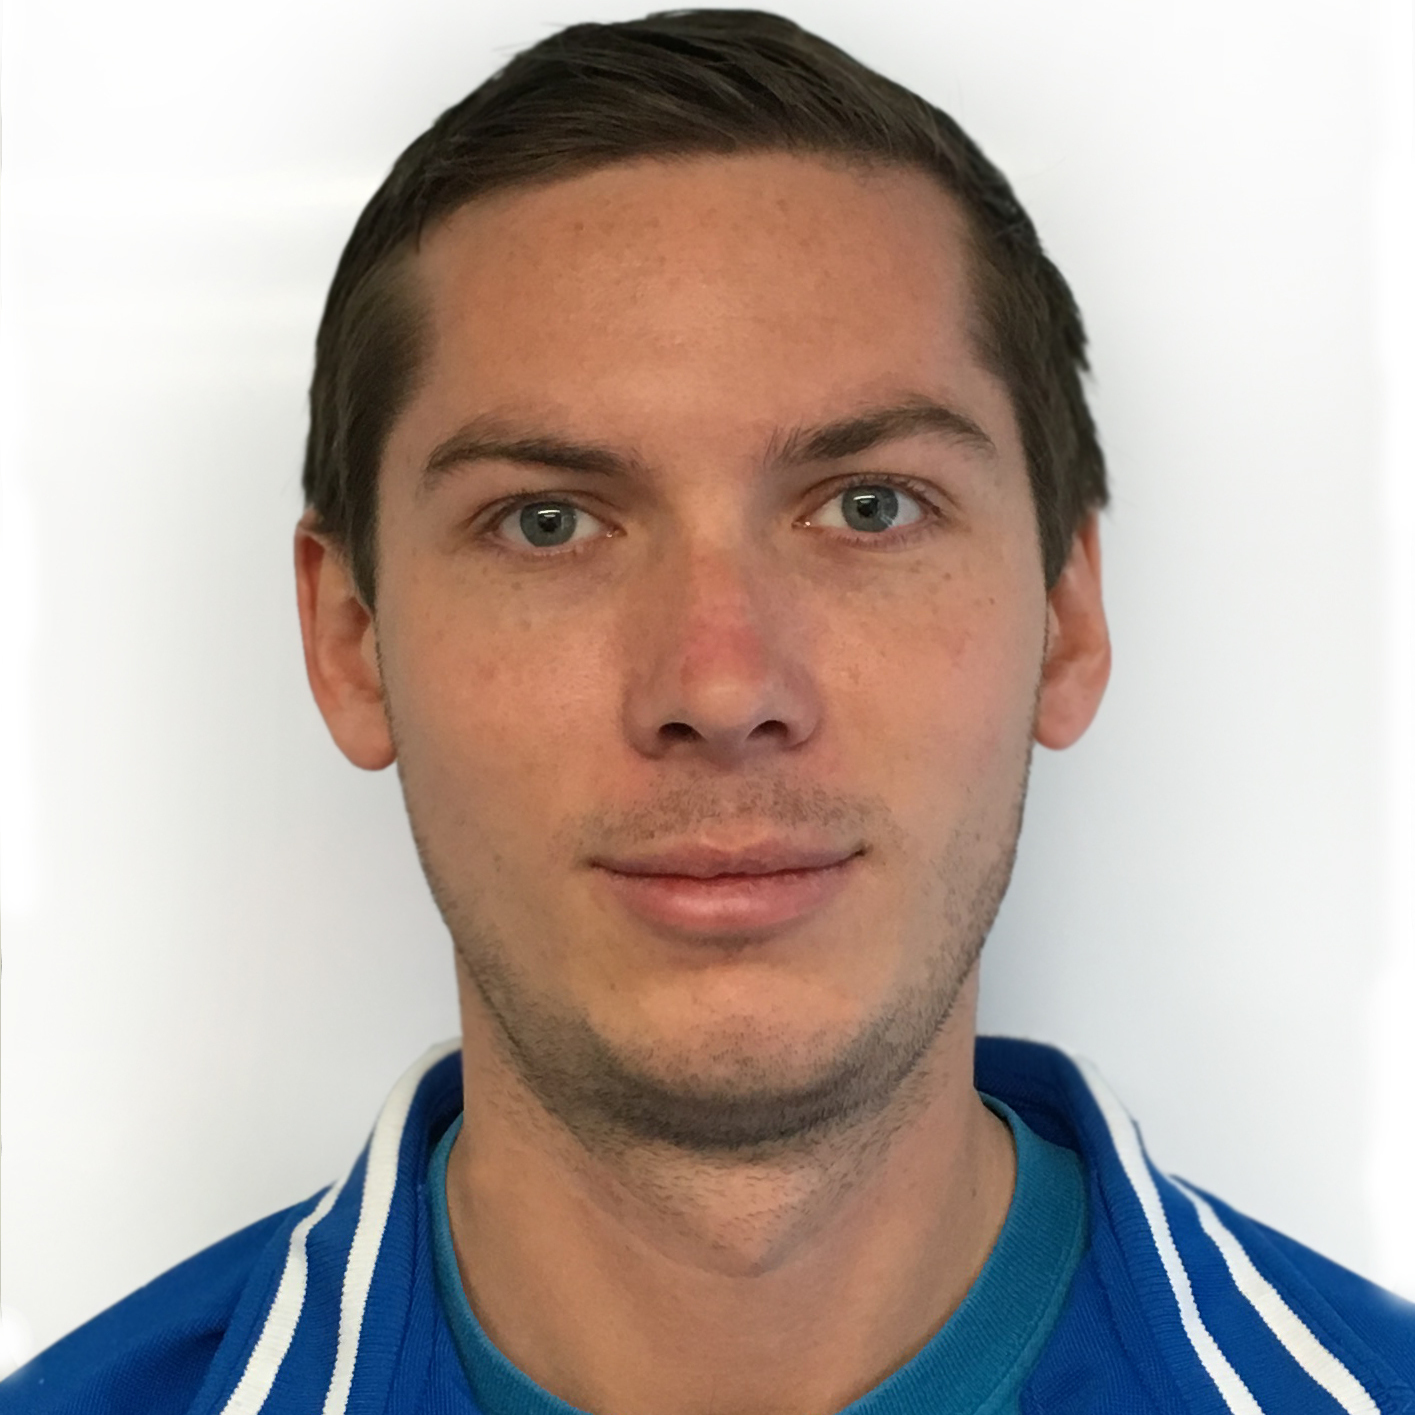
\includegraphics[width=0.48\linewidth]{oliver_sheridan_methven_picture_square}
	\end{minipage}
  }
  {
  	{\textsc{Improving performance with \\[0.1em] vectorised computations}}
 	}
  {
	\vspace{0.5em}
	{Oliver Sheridan-Methven} \\[0.1em]
	\texttt{oliver.sheridan-methven@maths.ox.ac.uk} \\[0.1em]
	Mathematical Institute, University of Oxford \\
  }
  {
    \begin{minipage}{0.25\linewidth}
      
\includegraphics[width=\linewidth]{infomm_logo_blue}
    \end{minipage}
    
  }


  \headerbox{Vectorised operations}{%
  	name=vectorisedOperations,span=2,column=0,row=0}
  {

%When computers operate on data, the instructions forming an operation are done one after another. Once an operation is finished on one piece of data, it's repeated on the next, in a procedure known as \textit{scalar} processing. Modern processors though can perform operations in parallel on large batches of data. Provided there is only a single set of instructions determining the data processing, then the operation is known as a \textit{single instruction multiple data} (SIMD) operation.
%	
%To perform these SIMD operations, processors have \textit{vector} capabilities. Upcoming \arm designs will use the \textit{scalable vector extension} (SVE) architecture \citep{stephens2017arm} depicted in \Cref{fig:sve_registers}, while \intel currently uses the \textit{advanced vector extension} (AVX) architecture. \arm architectures will offer vector lengths as multiples of 128-bits between \mbox{128--2048-bits}, whereas \intel's AVX\,512 has vectors fixed at 512-bits, (also shown in \Cref{fig:sve_registers}).

\begin{Figure}
	\centering
	\missingfigure[figwidth=\linewidth]{sve registers} \\[1em]
	\missingfigure[figwidth=\linewidth]{vectorised registers}
	\captionof{figure}{\textbf{(Top)}~\arm's SVE architecture showing predicate and vector registers. \textbf{(Bottom)}~An AVX 512-bit vector register containing $ n $ data elements.}
	\label{fig:sve_registers}
\end{Figure}


Vector operations are not without their drawbacks. Aside from difficulties removing intra-vector dependencies, conditional operations reduce performance \citep[pg.\,22--27]{loshin2001efficient}. For scalar operations the processor will evaluate the condition, and perform only the one required computation. However, for a SIMD operation, because some vector elements may require different branches of the condition, both computations are performed. Using the predicating registers one result is selected, but redundant calculations are performed, as depicted in \Cref{fig:simd_branching}.


\begin{Figure}
	\centering
	\missingfigure[figwidth=\linewidth]{simd branching}
	\captionof{figure}{\textbf{(Left)} Scalar handling of conditional statements. \textbf{(Right)} SIMD conditional processing.}
	\label{fig:simd_branching}
\end{Figure}

}



  \headerbox{Sobol scrambling}
  {name=sobolScrambling, column=0, below=vectorisedOperations, row=0, span=2}
  {

	Sobol sequences are \textit{low discrepancy} quasi-random numbers \citep[5.2.3]{glasserman2013monte}. These are heavily utilised in quasi-Monte Carlo applications, where using $ N $ samples from a Sobol sequence decreases the Monte Carlo error as $ N^{-1} $, (improving on $ N^{\nicefrac{-1}{2}} $). However, to recover a confidence interval the sequence must be \textit{randomised}, one method being \textit{digital scrambling}. 

			\begin{wrapfigure}{R}{0.4\linewidth}
					\noindent\centering
\raisebox{-0.5em}[0cm][5mm]{\begin{minipage}[c][0.1cm][c]{\linewidth}
				\begin{alignat*}{2}
				s_i           & =  0.8_{10}      \: & = 0.110011001100_2\cdots  &\\
				r             & =  0.\dot{3}_{10} & = 0.010101010101_2\cdots  &\\
				\tilde{s}_i \coloneqq s_i \veebar r & =  0.6_{10}       & = 0.100110011001_2\cdots  &
				\end{alignat*} 
\end{minipage}}
			\end{wrapfigure} 			
	Given $ m $ quasi-random numbers $ \{s_i\}_{i=0}^{m-1} \in [0, 1)$, we digitally scramble these by taking the \textit{bit-wise} \textit{exclusive OR} ($\textrm{XOR} \equiv \veebar  $) with a randomisation number $ r \in [0, 1)$. This produces the scrambled sequence $ \{\tilde{s}_i\}_{i=0}^{m-1} \in [0, 1)$.

		
	A feature of Sobol sequences is that for a sequence of $ m < 2^{k+1} $ terms (where $ k \in \mathbb{N}^0 $), the binary representations are non-zero in at most the first $ k + 1 $ digits following the radix \citep[3.2.2]{gentle2005random}.
	Furthermore, random number generators typically generate integers \citep[4.2.1]{tezuka1995uniform} normalised by $ 2^{32}$ \citep[1.3.2, pg.\,172]{gentle2005random}. So provided $ m < 2^{31} $, both the randomisation number and Sobol element can be stored in a 32-bit memory address.  


  }
  
  \headerbox{Vectorised digital scrambling}{name=vectorisedDigitalScrambling, column=2, span=2}
  {
  	

  		  	
	  	A difficultly in digital scrambling is reformatting the memory representation of the random number for the bit-wise XOR operation. Given the random number $ x \in (0, 1) $ is in floating-point format, then it's stored using scientific notation  $ x  \equiv \pm (1.a_1a_2\cdots a_m)_2 \times 2^{(b_1b_2\cdots b_e)_2} $. We store $ m + 1 $ significant figures (the \textit{mantissa}),  $ e $ digits of the exponent, and use a single bit for the sign,  (\Cref{fig:floating_point_representation} shows how this is stored in memory). Scrambling can then be performed by one of two methods: \\
\begin{minipage}[t]{\linewidth}
\centering
\begin{minipage}[t]{0.4\linewidth}
\begin{enumerate}[a)]
\item Multiply by $ 2^{32} $.
\item Convert into an unsigned integer. 
\item Bit-wise XOR. 
\item Convert back to a float. 
\item Multiply by $ 2^{-32} $. 
\end{enumerate}
\end{minipage} 
\begin{minipage}[t]{0.4\linewidth}
\begin{enumerate}[i)]
\item Multiply by $ 0.5 $ and add $ 0.5 $. 
\item Bit-wise XOR. 
\item Bit-wise XOR with $ 0.5 $. 
\item Multiply by 2 and subtract 1. 
\end{enumerate}
\end{minipage} 
\end{minipage}

  		
	  	\begin{Figure}
	  		\centering
	  		\missingfigure[figwidth=\linewidth]{floating point representation}
	  		\captionof{figure}{The representation in memory of a floating-point number.}
	  		\label{fig:floating_point_representation}
	  	\end{Figure}
  		
  		
  		\begin{wrapfigure}{l}{0.42\linewidth}
  			\centering
  			\raisebox{-5mm}[0cm][40mm]{
  				\centering\noindent
  				\begin{minipage}[t]{0.95\linewidth}
  				\centering
  			\begin{tabular}{|cc>{$}c<{$\,\%}|}
  				\hline
  				\rowcolor{oxford_blue} \textcolor{white}{Precision} & \textcolor{white}{Digits} & \multicolumn{1}{c|}{\textcolor{white}{Improvement}} \\ \hline
  				Double & 32 & +530 \\
  				Single & 32 & -280 \\
  				Single & 23 & +120 \\
  				\hline 
  			\end{tabular}
  			\captionof{table}{The speed difference when using the ``scientific notation'' scrambling implementation over the ``integer conversion'' method. We include the case when there are at most 23 non-zero digits immediately after the radix.}
  			\label{tab:performance_times_scientific_vs_integer}
  			\end{minipage}
  		} \hfill 
  		\end{wrapfigure}
  		A 32-bit floating-point number's mantissa is 23-bits, so trying to keep the number in scientific notation will cause underflow to zero for numbers less than $ 2^{-23} $. To maintain correctness our SIMD implementation required considerably more floating-point manipulations. However, if we relax our assumption of 32 possibly non-zero digits down to 23, then we can perform the same procedure as for 64-bit floats. Scrambling $ 10^9 $ random numbers and comparing the vectorised ``integer conversion'' and ``scientific notation'' approaches gave the results shown in \Cref{tab:performance_times_scientific_vs_integer}. 
  		
  		
  	}

  \headerbox{Inverse Gaussian cumulative density function $ \Phi^{-1} $}
  {name=inverseCDF, column=2, span=2, below=vectorisedDigitalScrambling}
  {
  	  	
  	  	Frequently we require random numbers from a Gaussian distribution, which involves transforming a uniformly distributed random variable. If quasi-Monte Carlo is desired, a Sobol sequence can be transformed using the \textit{inverse cumulative density function method} \citep[2.2.1]{glasserman2013monte}. 
  	  	
  	  	\begin{wrapfigure}{l}{0.35\linewidth}\centering
  	  		\raisebox{10mm}[0cm][62mm]{
  	  			\begin{minipage}[t]{0.99\linewidth}
			\begin{equation}
  	  		\label{eqt:def:inverse_cdf_gaussian}
  	  		\dfrac{1}{\sqrt{2\pi}}\! \int\displaylimits_{-\infty}^{\Phi^{-1}(x)}\! \exp(\dfrac{-\xi^2}{2}) \dd{\xi} = x
  	  		\end{equation}
  	  		\centering
  	  		\missingfigure[figwidth=\linewidth]{inverse cdf function shrunk}
  	  		\captionof{figure}{The inverse Gaussian CDF function $ \Phi^{-1}(\cdot) $.}
  	  		\label{fig:inverse_cdf_function}
  	  			\end{minipage}
  	  		} 
  	  	\end{wrapfigure}
  	  	If $ x $ is a uniformly distributed random number, and $ \Phi^{-1}(\cdot) $ is the inverse cumulative density function (CDF) of the Gaussian distribution as given in \Cref{eqt:def:inverse_cdf_gaussian}, then $ \Phi^{-1}(x) $ follows a standard Gaussian distribution.   	  	
  	  	While \Cref{eqt:def:inverse_cdf_gaussian} looks intractable, it can be approximated to machine precision by either a polynomial or Pad\'{e} approximation, as done by \citet{evans1974algorithm70}. Extensions to full double-precision \citep{beasley1985percentage,wichura1988algorithm,marsaglia1994rapid}  are achieved by splitting $ \Phi^{-1}(\cdot) $ into an cheap central region, and a more expensive tail region at the asymptotes, (cf. \Cref{fig:inverse_cdf_function}). The tail regions require the more costly evaluations of logarithms and square roots.
  	  	
  	  	We benchmarked several methods for evaluating  $ \Phi^{-1}(\cdot) $  using the Intel \textit{vector statistics library} (VSL) and the \textit{GNU  scientific library} (GSL). We also included a vectorised modification of the \textit{inverse error function} $ \textrm{erfinv}(\cdot) $, as proposed by \citet{giles2011approximating}. All possible inputs and exceptions were correctly handled, and precision maintained. The results are shown in \Cref{fig:inverse_cdf_performance}, where we include the average time for reading and writing, and $ \sin(\cdot) $. The inputs extend down to $ 10^{-20} $, and include zero, one, and NaN. 
			\begin{Figure}
				\centering
				\missingfigure[figwidth=\linewidth]{intel inverse cdf performance}
				\captionof{figure}{A comparison of double-precision $ \Phi^{-1}(\cdot) $ implementations by Intel, GNU, and \citet{giles2011approximating}. \intel implementations for low and high-accuracy modes are shown. Averages for NaN input are shown on the right. Averages for random input are shown as solid lines on the left, with empirically expected averages shown as dashed lines. These data were gathered using a 64-bit x86 \intel Xeon Gold 6140 CPU operating at 2.3\,\si{\giga\hertz} under GNU/Linux 4.13.0-25-generic under the Ubuntu 16.04.3 LTS distribution. C code was compiled using the Intel C compiler 18.0.0 with the flags \texttt{-qopenmp}, \texttt{-std=c11}, \texttt{-mkl}, and \texttt{-O2}.}
				\label{fig:inverse_cdf_performance}
			\end{Figure}


  }

  \headerbox{Acknowledgements}
  {name=acknowledgements, column=0, above=bottom, span=2}
  {
  	\begin{center}
  		\begin{minipage}[t]{0.95\linewidth}
  			
\includegraphics[width=0.3\linewidth, valign=t]{epsrc_logo} 
  			\hfill
  			
\includegraphics[width=0.3\linewidth, valign=t]{arm_logo_blue}
  			\hfill
  			
\includegraphics[width=0.23\linewidth, valign=t]{nag_logo_blue}
  		\end{minipage}
  	\end{center}
  	
  }


\headerbox{References}
{name=references, column=0,  below=sobolScrambling, above=acknowledgements, span=2}
{
	\renewcommand{\section}[2]{\vspace{0.05em}} % Omit "References" title

	\begin{multicols}{2}
		\bibliography{../thesis/references}
	\end{multicols}

}


\end{poster}

\end{document}


